%%
%% Author: dariochinelli
%% 2021-04-05
%%


\section{Diffrazione raggi X}
Nel 1913 Bragg scoprì che i solidi cristallini producono pattern molto particolari nella diffrazione di raggi $X$.
Scoprì infatti che i cristalli, a determinate lunghezze d'onda, producono picchi di intensità di radiazione diffusa ad angoli ben precisi.

\paragraph{Cos'è un \textit{reticolo cristallino}?} 
Si consideri ad esempio un pezzo di ferro, gli atomi che lo compongono sono localizzati nello spazio in una struttura ordinata, esso possiede un \textit{ordine cristallino}.
È come avere una matrice di atomi, posti in posizioni ben precise e ripetute "infinitamente", semplificando la trattazione, consideriamo celle di forma cubica.

\paragraph{Irraggiamento di un cristallo}
Per angoli ben precisi si osservano picchi della radiazione, dovuti all'interferenza costruttiva di due onde \textit{riflesse} da due diversi piani atomici dell struttura cristallina.
Questo concetto venne spiegato da Max Von Laue.
Pensando ad un reticolo di diffrazione: ogni fenditura è sorgente di onde,
allo stesso modo ogni atomo si comporta come una sorgente d'onde e si verifica l'interferenza costruttiva.
\begin{figure}[h]
\centering
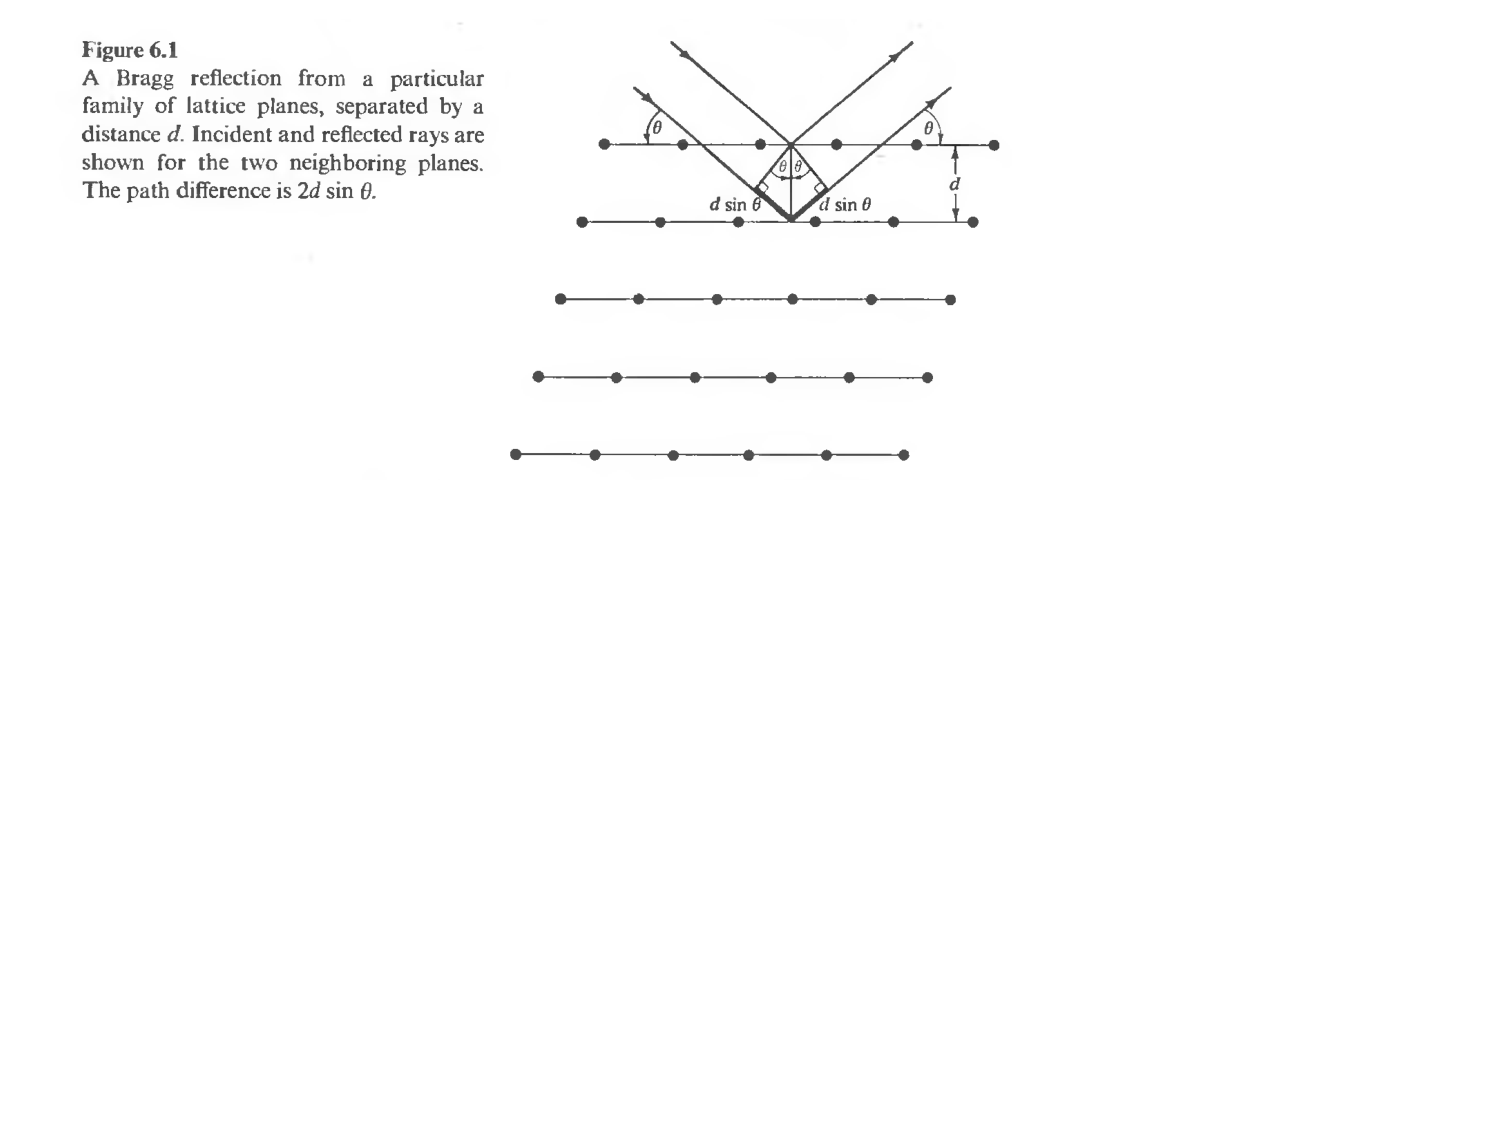
\includegraphics[scale=0.7]{/atomi_radiazineX}
\caption{Diagramma dei piani atomici di un cristallo}
\end{figure}

Il contributo fondamentale per capire il fenomeno fu dato da William Henry Bragg e da William Lawrence Bragg, padre e figlio, i quali conoscendo i lavori di Von Laue capirono che si poteva spiegare il fenomeno assumendo che: \\ 
\textit{"per ogni raggio diffratto esiste un set di piani reticolari cosicché il raggio diffratto appare come riflesso specularmente da tale set di piani"}. \\

\begin{figure}[h]
\centering
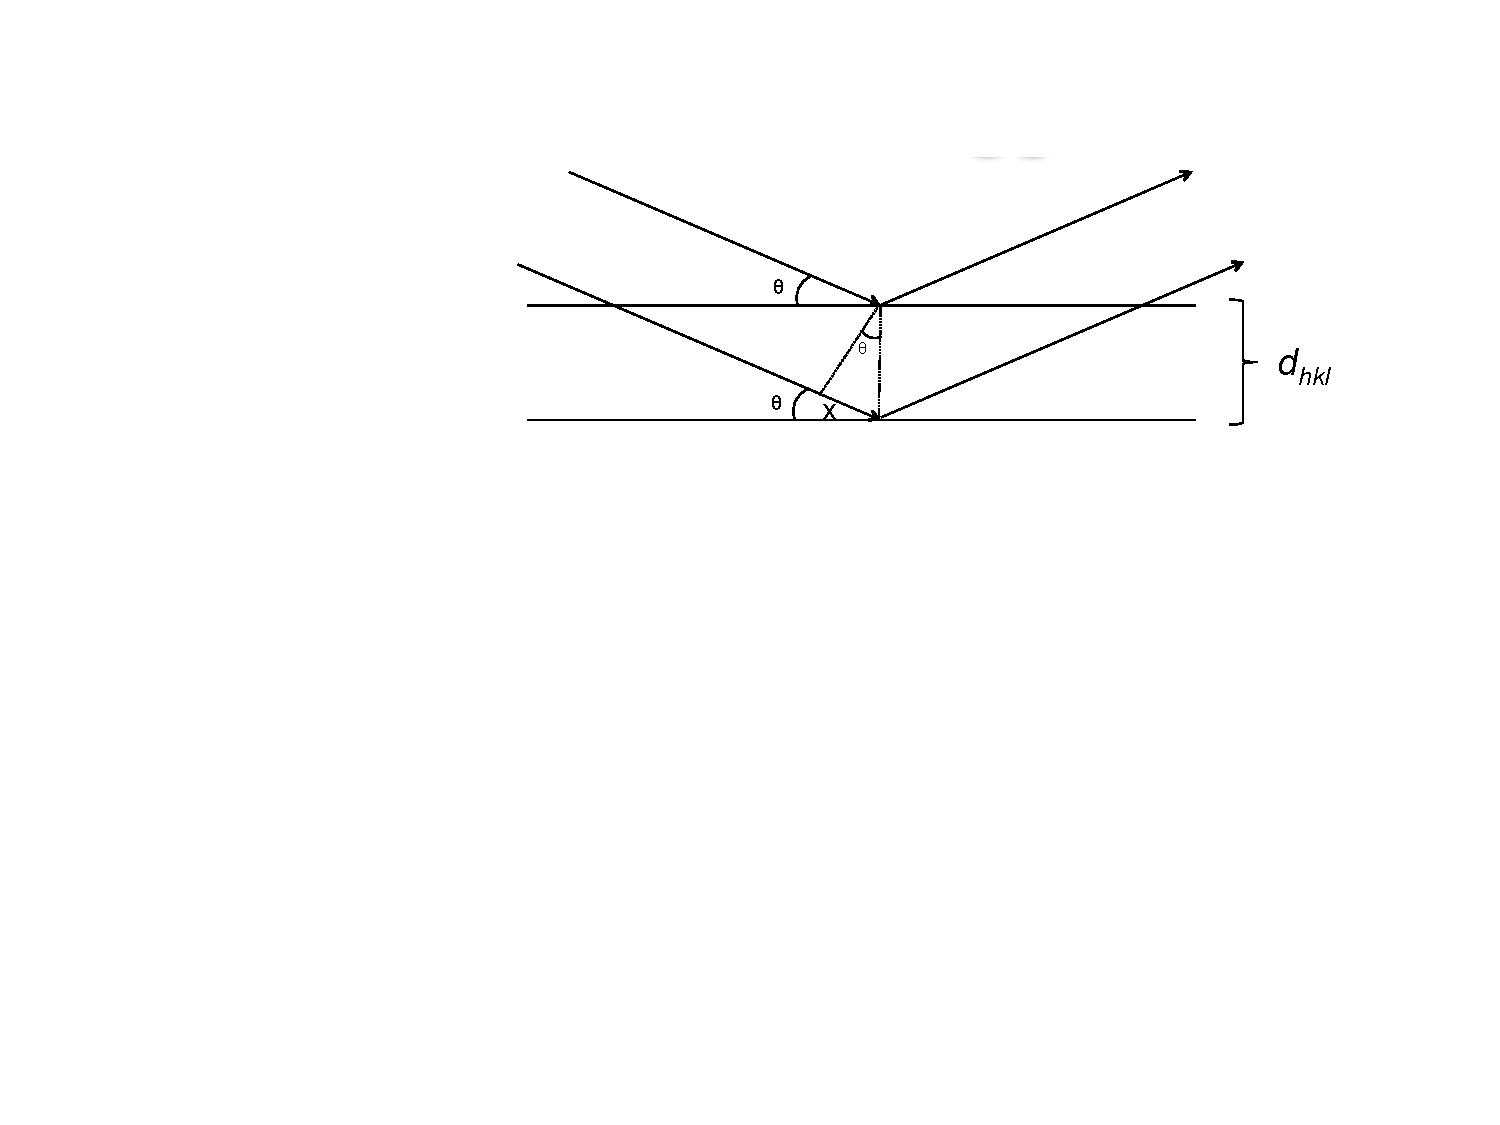
\includegraphics[scale=0.7]{/schema_bragg}
\caption{Schema cammini ottici}
\label{cammino_ottico}
\end{figure}

\textbf{L'ipotesi di Bragg} è che i piani siano semi-riflettenti.
Come si vede in figura \ref{cammino_ottico} la differenza di cammino ottico sarà data da
\begin{equation}
\begin{split}
& \Delta = 2 (d \sin\theta) \\ 
& 2 d \sin\theta = n \lambda 
\end{split}
\end{equation}
Dove l'ultima equazione è la parte analitica della \textbf{Legge di Bragg}. \\
Bragg interpreta il fenomeno come una riflessione e non come una diffrazione, quando è verificata la condizione precedente.
Significa quindi che si tratta di picchi di \textit{riflessione} detti "picchi di riflessione di Bragg".
Per ogni tipo di cristallo potrò osservare tanti picchi di diffrazione ad angoli diversi, che corrispondono ad una riflessione da un set reticolare diverso.
Questo fenomeno è utile per investigare la materia:
sottoponendo un campione ad un fascio di raggi X risalgo alla sua struttura cristallina attraverso l'osservazione del pattern di diffrazione ottenuto.

\begin{figure}[h]
    \centering
    \subfloat[Picchi di intensità per un materiale cristallino con struttura cubica]{
        \label{es_diff_1}
        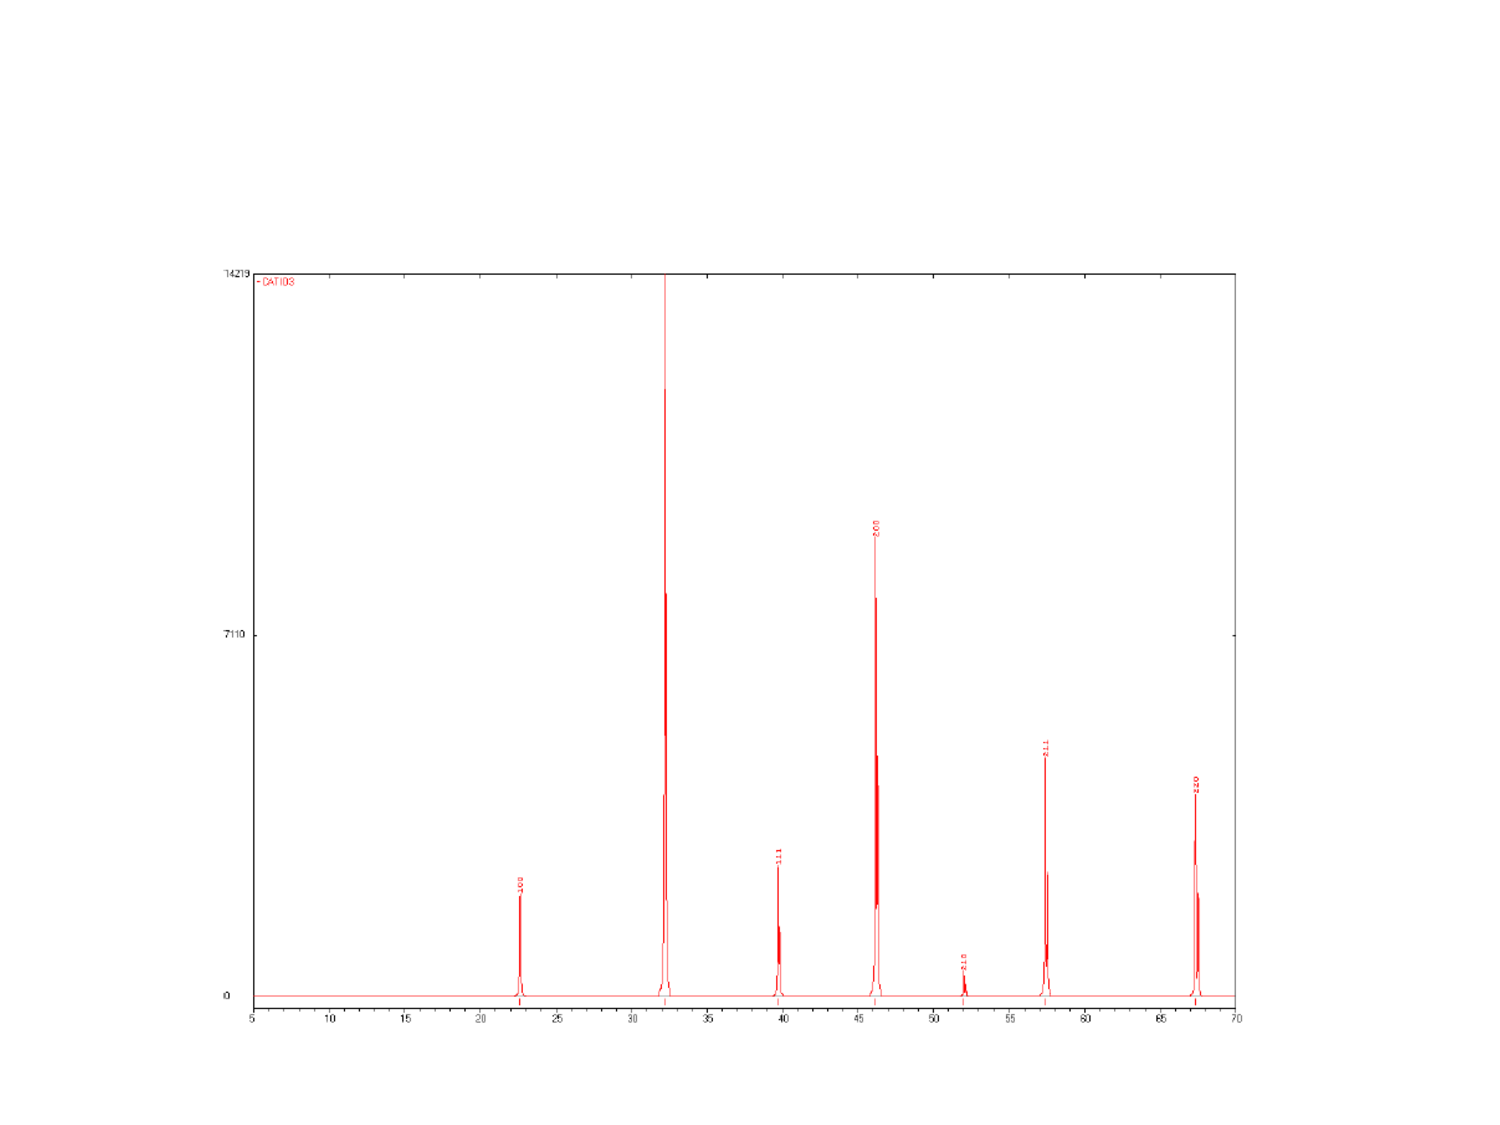
\includegraphics[width=0.5\textwidth]{/diffusione_raggiX}
    }
    \subfloat[Spettro di diffrazione in funzione dell'angolo]{
        \label{es_diff_1}
        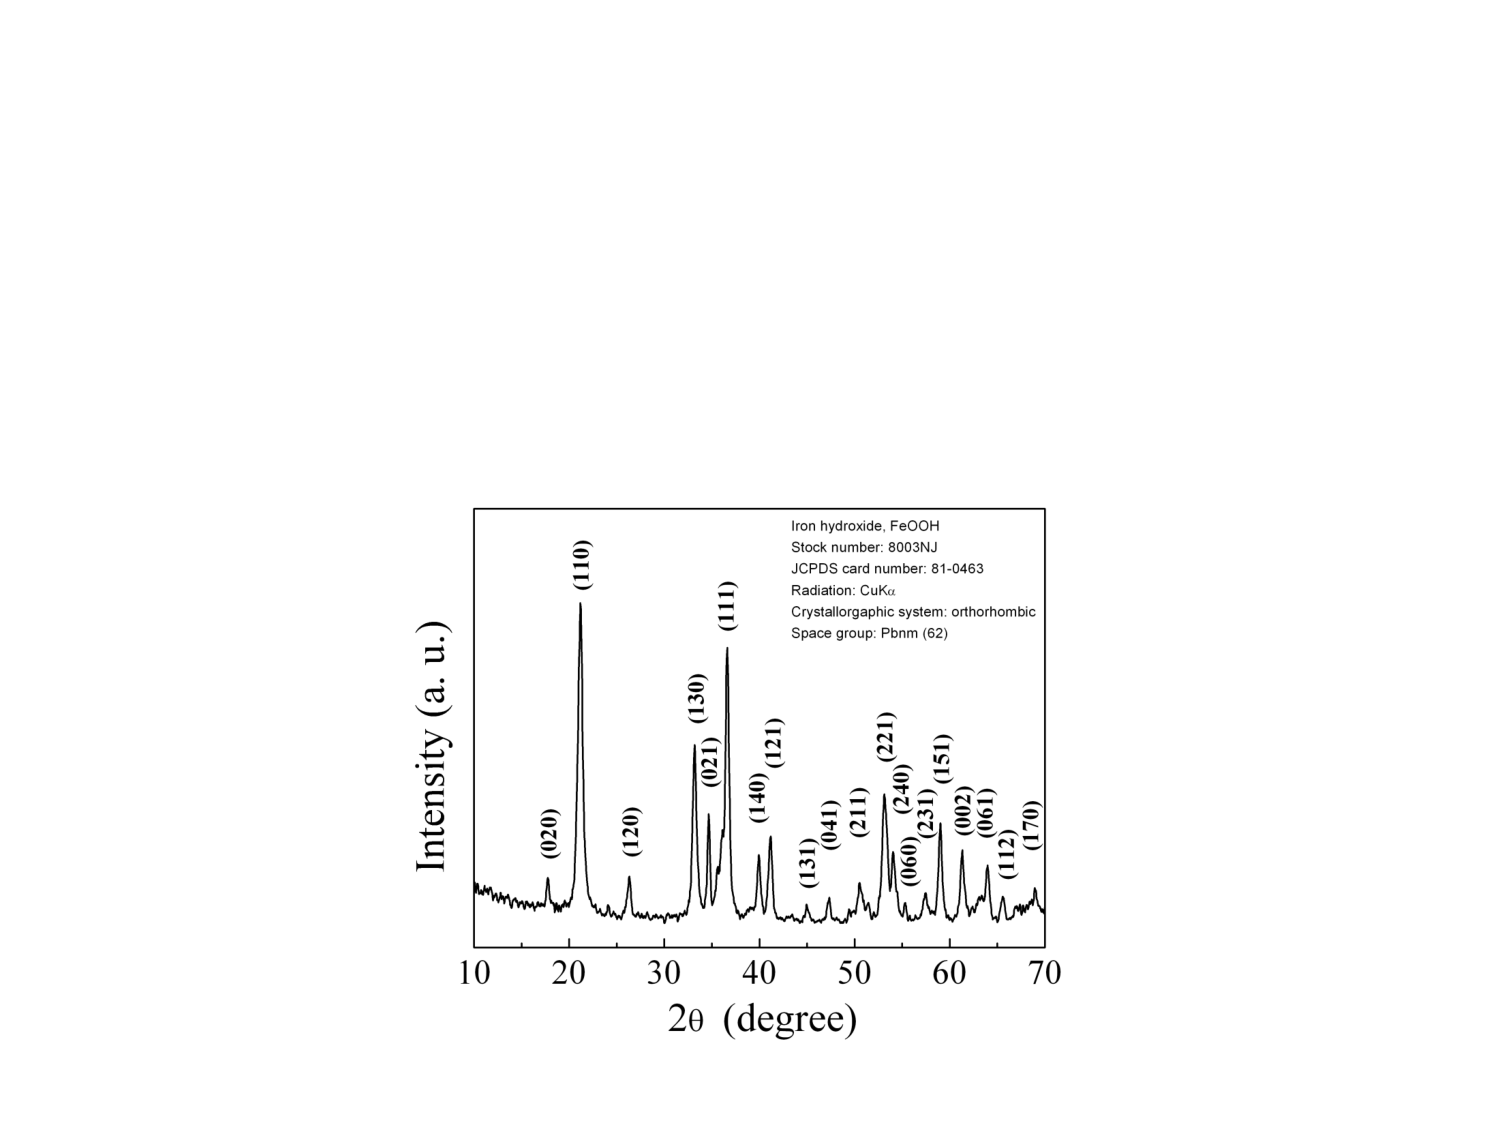
\includegraphics[width=0.5\textwidth]{/pattern_diffrazione_X}
    }
    \caption{Esempi di spettri di diffrazione}
    \label{es_diff}
\end{figure}
